
\documentclass[master]{thesis-uestc}

\title{基于穿戴式IMU的老年人运动监测系统研究}{The Time Marching Scheme of Time Domain
    Integral Equation and Corresponding Fast ???????????}

\author{陈泳吉}{Chen Yongji}
\advisor{周军\chinesespace 教授}{Dr. Jun Zhou}
\school{信息与通信工程学院}{School of Physical Electronics}
\major{电子与通信工程}{Radio Physics}
\studentnumber{201952011735}

% require all the usepackages here
% \usepackage{algorithm2e}

\begin{document}

\makecover

% This is a template of mutiple files.
% The folders chapters/ and misc/ have the related files

% abstract
	
\begin{chineseabstract}
为了适应日益增长的宽带信号和非线性系统的工程应用,用于分析瞬态电磁散射问题的时域积分方程方法研究日趋活跃。本文以时域积分方程时间步进算法及其快速算法为研究课题,重点研究了时间步进算法的数值实现技术、后时稳定性问题以及两层平面波算法加速计算等,主要研究内容分为四部分。

……

\chinesekeyword{时域电磁散射,时域积分方程,时间步进算法,后时不稳定性,时域平面波算法}
\end{chineseabstract}



\begin{englishabstract}
	With the widespread engineering applications ranging from broadband signals and non-linear systems, time-domain integral equations (TDIE) methods for analyzing transient electromagnetic scattering problems are becoming widely used nowadays. TDIE-based marching-on-in-time (MOT) scheme and its fast algorithm are researched in this dissertation, including the numerical techniques of MOT scheme, late-time stability of MOT scheme, and two-level PWTD-enhanced MOT scheme. The contents are divided into four parts shown as follows.
	
	\englishkeyword{time-domain electromagnetic scattering, time-domain integral equation (TDIE), marching-on in-time (MOT) scheme, late-time instability, plane wave time-domain (PWTD) algorithm}
\end{englishabstract}




% table of contents
\thesistableofcontents

% thesis contents
\chapter{绪\hspace{6pt}论}

\section{研究工作的背景与意义}

计算电磁学方法\citing{wang1999sanwei, liuxf2006, zhu1973wulixue, chen2001hao, gu2012lao, feng997he}从时、频域角度划分可以分为频域方法与时域方法两大类。频域方法的研究开展较早,目前应用广泛的包括:矩量法(MOM)\citing{xiao2012yi,zhong1994zhong}及其快速算法多层快速多极子(MLFMA)\citing{clerc2010discrete}方法、有限元(FEM)\citing{wang1999sanwei,zhu1973wulixue}方法、自适应积分(AIM)\citing{gu2012lao}方法等,这些方法是目前计算电磁学商用软件
\footnote{脚注序号“\ding{172},……,\ding{180}”的字体是“正文”,不是“上标”,序号与脚注内容文字之间空1个半角字符,脚注的段落格式为:单倍行距,段前空0磅,段后空0磅,悬挂缩进1.5字符;中文用宋体,字号为小五号,英文和数字用Times New Roman字体,字号为9磅;中英文混排时,所有标点符号(例如逗号“,”、括号“()”等)一律使用中文输入状态下的标点符号,但小数点采用英文状态下的样式“.”。}
(例如:FEKO、Ansys 等)的核心算法。由文献\cite{feng997he,clerc2010discrete,xiao2012yi}可知

\section{时域积分方程方法的国内外研究历史与现状}
时域积分方程方法的研究始于上世纪60 年代,C.L.Bennet 等学者针对导体目
标的瞬态电磁散射问题提出了求解时域积分方程的时间步进(marching-on in-time,
MOT)算法。

\section{本文的主要贡献与创新}
本论文以时域积分方程时间步进算法的数值实现技术、后时稳定性问题以及两层平面波加速算法为重点研究内容,主要创新点与贡献如下:

\section{本论文的结构安排}
本文的章节结构安排如下:




\chapter{运动监测相关原理}
运动监测技术就是通过视觉或者传感器的数据,来估计用户的运动情况。在前文中,我们已经介绍HAR可以分为两类:基于视觉的HAR和基于穿戴式传感器的HAR。
基于视觉的HAR有许多局限性,例如摄像头等可视化工具通常是被固定的,更适合在室内使用,对于贯穿室内外以及不同地点的行为存在诸多限制,同时受光照、拍摄角度以及环境噪声的影响,难以提高分类精度。
与基于视觉的HAR相比,基于传感器的可穿戴HAR不受上述噪声的影响,可以实现更高的精度。
本章主要介绍基于穿戴式IMU的运动监测原理。


\section{人类活动识别原理}
\subsection{人类活动分类概述}



\subsection{常用算法}
\subsubsection{卷积神经网络}

\section{跌倒检测原理}
\subsection{跌倒过程}


\subsection{跌倒检测评估方法}
\subsection{常用算法}
\subsubsection{支持向量机算法}




\section{数据集}

\section{本章小结}




% \section{传感器及其应用简介}
% 论文主要涉及到三种传感器:加速度计、陀螺仪和气压计。为满足研究中传感器的要求,本文中所使用的IMU为维特智能公司生产的型号为HWT901B的集成传感器模块,包含三轴加速度计、三轴陀螺仪、三轴磁力计和气压计,
% 如图\ref{imu}所示。本文中使用的都是微机电系统(Micro­Electro Mechanical Systems,MEMS)下的传感器,由于构成原理和制作工艺等方面的因素,MEMS 传感器具有更多良好的特性,如成本低、可靠性高、功耗低和体积小等等优点。在介绍具体算法之前,本节先对这三种传感进行简单介绍。

% 	\begin{figure}[h]
% 		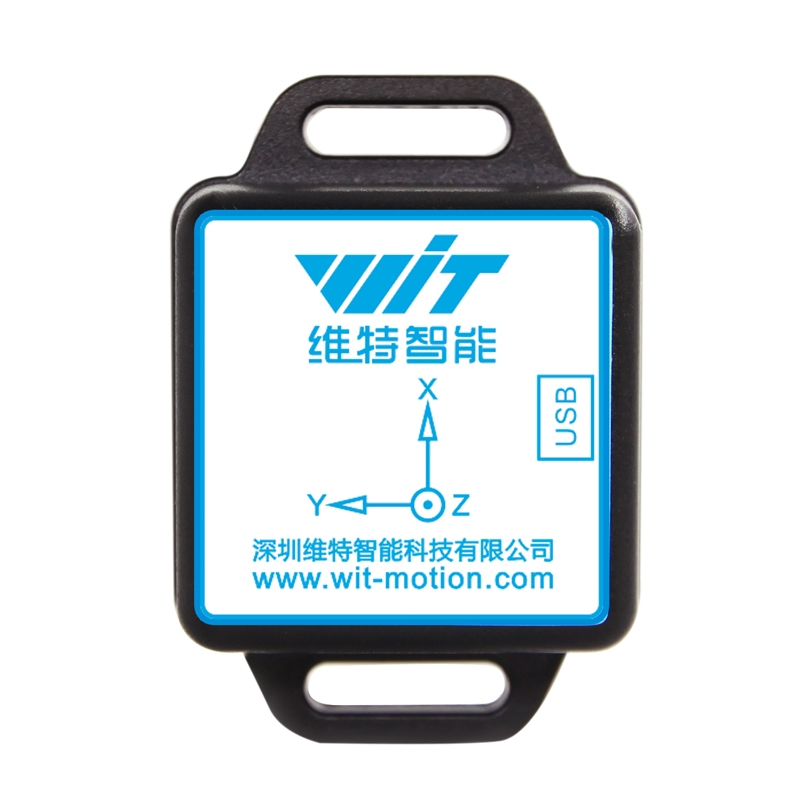
\includegraphics[width=0.3\textwidth]{IMU.jpg}
% 		\caption{RWG 基函数几何参数示意图}
% 		\label{imu}
% 	\end{figure}


% \subsection{加速度计}
% % 可以借用  基于改进CNN-LSTM的人体行为识别研究_龙秋玲  中2.1.1

% 加速度计是一种惯性传感器,它能够测量物体的加速度。当加速度计与物体一起运动时,能够将加速度转化为输出信号。目前常用的是MEMS加速度计,由于采用了微机电系统技术,使得其尺寸大大缩小,一个MEMS加速度计只有指甲盖的几分之一大小。MEMS加速度计具有体积小、重量轻、能耗低等优点。

% 本文所用到是三轴加速度计,三个轴的方向互相垂直构成一个空间直角坐标系,即加速度计的输出分别是载体在空间相互垂直的三个方向上的数据。因此,当加速度计静置于水平地面上时,由于加速度计本身与地面相对静止,加速度计三轴的一个必定与地面垂直,如图\ref{acc}所示。此时加速度计仅受到地心引力的作用,因此其三轴输出中,仅有跟地面垂直的那个轴有读数,而且读数的绝对值应该是在重力加速度 g 附近小幅度波动,而另外两个轴的读数应该是在 0 附近小幅度波动,这种波动产生则是由传感器本身以及周围的环境噪声引起的。

% \begin{figure}[h]
% 	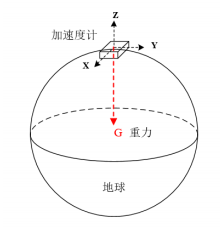
\includegraphics[width=0.3\textwidth]{acc.jpg}
% 	\caption{RWG 加速度计静置与水平地面示意图}
% 	\label{acc}
% \end{figure}

% % 由于重力加速度的存在,静置于水平地面的加速度计的垂直于水平面的轴的读数正好是重力加速度g,利用这种特性,当加速度计至于非水平地面上时,重力的方向将不再与原轴重合,而是可以将其以某个角度分解至两个轴上,如图 2­2 所示。因此可以通过加速度计三轴的读数,结合三角函数即可得到加速度计当前所处位置与水平面所成的角度关系。 田园师兄论文出处

% 将加速度计放在人身上,人体在日常生活中会不断做出各种动作,加速度会伴随动作一起出现,利用加速度计采集这些加速度信息就可以得到人体运动的加速度信息,通过科学的方法进行处理和分析,就可以用来监测人们的日常行为,从而更好的改善人们的生活。


% \subsection{陀螺仪}

% 可能涉及不到,暂定!

% \subsection{气压计}
% % 可以借用 基于智能手机多传感器融合技术的人体活动识别研究_杨佳现   中2.2.2  章内容
% 气压传感器主要用于测量大气压强,气压国际制单位是帕斯卡,简称帕,符号是Pa。其中MEMS气压传感器主要原理是压电效应,压电材料可以产生电流。当它们受到外力的作用时,材料会产生形变,其内部会产生极化现象,在形变的两端出现正负等量的电荷。首先,电流可以用来计算材料的形变程度,然后材料的形变可以用来计算外力大小,因此探测电流就可以计算出外力大小。

% 这类MEMS压力传感器本质上是一个空气腔,其一侧带有类似气球的柔性材料。当传感器位于气压较高的区域(例如低谷)时,膜就会由于外界压力变大而被推向腔内。当传感器位于气压低的区域(例如山峰),膜会从腔体中凸出。在这层膜上附有敏感材料。传感器可以读取材料(形变)产生的电流变化,然后通过该电流读数计算出施加到膜上的压力。接下来,因为腔内的压力已知,那么传感器就可以计算出外部压力大小。

% 气压传感器用途广泛,用户通过气压传感器可计算得出测量设备所处的海拔高度,进而提高利用智能手机进行定位的可靠性和精准度,也可直接用来进行辅助设备的 GPS 定位,来帮助用户确认设备所在楼层的位置等相关信息。


% \section{基于IMU的运动监测技术}
% 基于IMU的运动监测技术的整个工作原理如下:首先从多个传感器收集数据,如加速度计、陀螺仪和气压计,这些传感器放置在大腿、腰部等,然后对数据进行滤波等处理,最后进行特征提取和分类。
% 在本文中,基于IMU的运动监测技术主要包含三个方面:人类活动识别、步行稳定性和跌倒检测。

% \subsection{人类活动识别}
% % 主要介绍目前有哪些方法可以进行识别,各有什么优点
% 人类活动识别主要是采集人类活动时的各种数据,通过某种方法,正确的分析出人类当前的运动状态,本文主要研究站立,走路,上楼,下楼这四个运动状态。在上一小节中,我们已经介绍了加速度计可以反映人体运动的加速度信息,所以可以根据加速度信息来对人类活动进行识别。

% 人类活动识别目前通用流程如图\ref{har1}所示,首先佩戴加速度传感器采集大量的活动数据,然后原始数据进行一系列的处理,由于数据中包含了各种各样的噪声,因此需要对原始数据进行预处理,例如分割和滤波等。预处理后的加速度数据经过特征选取组成特征矩阵,然后送入分类器进行模型训练和识别分类工作。训练好的模型将被用于识别过程中,在识别分类的时候,分类器需要用到待识别样本的特征矢量和之前训练好的分类模型,分类器会在两者么间进行匹配计算,使用特定的匹配算法,进而计算出两者之间的相似度,选出相似度最高的模板,将待识别样本归入到此类中,即得到了识别分类的结果。


% \begin{figure}[h]
% 	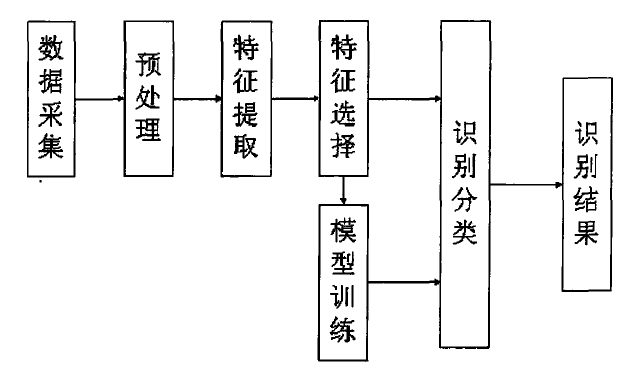
\includegraphics[width=0.5\textwidth]{har1.jpg}
% 	\caption{RWG 基于3轴加速度传感器的人体行为识别常用识别过程}
% 	\label{har1}
% \end{figure}

% \subsection{步行稳定性}
% \subsection{跌倒检测}

% % 参考论文   A Combined Smartphone and Smartwatch Fall Detection System

% 跌倒前阶段:受试者从事的日常生活的初始活动

% 自由落体阶段:由于失去平衡而向地面自由落体运动

% 撞击阶段:代表物体接触表面的那一刻的撞击

% 撞击后阶段:撞击后的瞬间,当人因跌落的冲击而躺在地板上时

% 恢复阶段:受试者努力站起来或从跌倒中恢复


% \section{本章小结}



% \subsection{空间基函数}
% RWG 基函数是定义在三角形单元上的最具代表性的基函数。它的具体定义如下:
% \begin{equation}
% f_n(\bm{r})=
% \begin{cases}
% \frac{l_n}{2A_n^+}\bm{\rho}_n^+=\frac{l_n}{2A_n^+}(\bm{r}-\bm{r}_+)&\bm{r}\in T_n^+\\
% \frac{l_n}{2A_n^-}\bm{\rho}_n^-=\frac{l_n}{2A_n^-}(\bm{r}_--\bm{r})&\bm{r}\in T_n^-\\
% 0&\text{otherwise}
% \end{cases}
% \end{equation}

% 其中,$l_n$为三角形单元$T_n^+$和$T_n^-$公共边的长度,$A_n^+$和$A_n^-$分别为三角形单元$T_n^+$和$T_n^-$的面积(如图\ref{pica}所示)。

% \begin{figure}[h]
% 	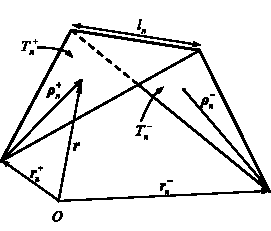
\includegraphics{pica.pdf}
% 	\caption{RWG 基函数几何参数示意图}
% 	\label{pica}
% \end{figure}

% 由于时域混合场积分方程是时域电场积分方程与时域磁场积分方程的线性组合,因此时域混合场积分方程时间步进算法的阻抗矩阵特征与时域电场积分方程时间步进算法的阻抗矩阵特征相同。
% \begin{equation}
% \label{latent_binary_variable}
% \bm{r}_{i,j}=
% \begin{cases}
% 1,f(\bm{x}^{i};\bm{w})\cdot f(\bm{x}^{j};\bm{w})\geq u(\lambda),\\
% 0,f(\bm{x}^{i};\bm{w})\cdot f(\bm{x}^{j};\bm{w})< l(\lambda), 1\leq i,j\leq n.\\
% f(\bm{x}^{i};\bm{w})\cdot f(\bm{x}^{j};\bm{w}),\text{otherwise},
% \end{cases}
% \end{equation}

% 时域积分方程时间步进算法的阻抗元素直接影响算法的后时稳定性,因此阻抗元素的计算是算法的关键之一,采用精度高效的方法计算时域阻抗元素是时域积分方程时间步进算法研究的重点之一。


% \subsection{时间基函数}

% \subsubsection{时域方法特有的展开函数}

% \subsubsection{频域方法特有的展开函数}

% \section{入射波}

% 如图\ref{picb}和图\ref{picc}所示分别给出了参数$E_0=\hat{x}$,$a_n=-\hat{z}$,$f_0=250MHz$,$f_w=50MHz$,$t_w=4.2\sigma$时,调制高斯脉冲的时域与频域归一化波形图。

% \begin{figure}[h]
% \subfloat[]{
% 	\label{picb}
% 	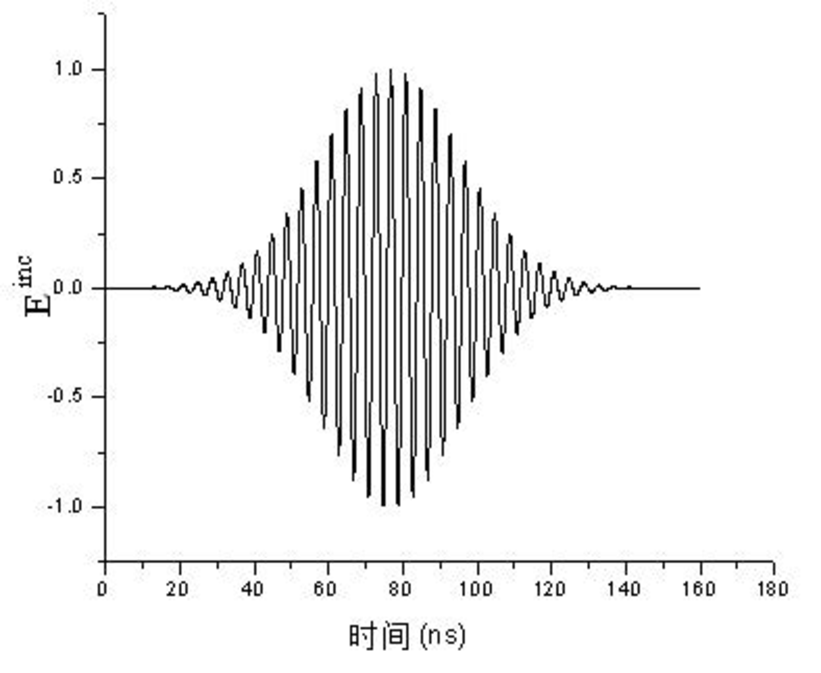
\includegraphics[width=7.3cm]{picb.pdf}
% }
% \subfloat[]{
% 	\label{picc}
% 	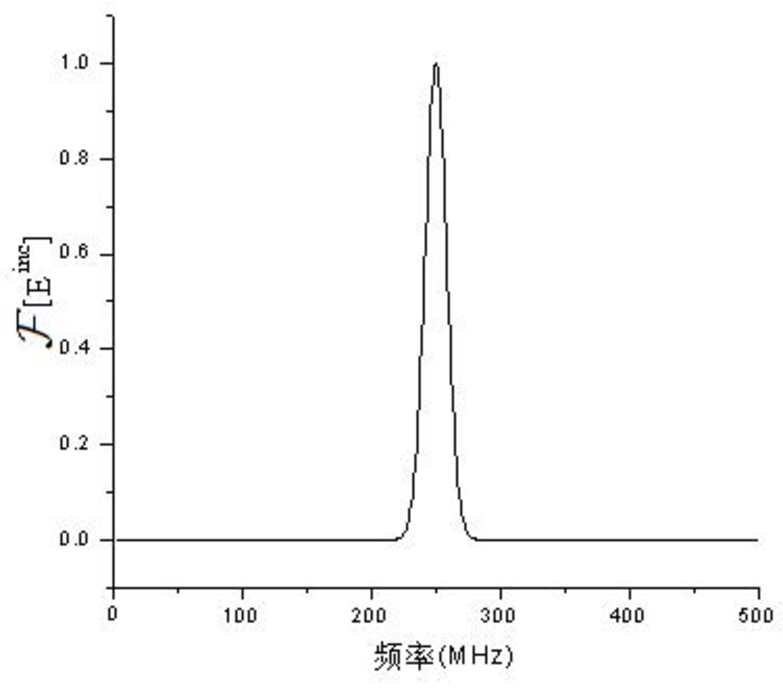
\includegraphics[width=6.41cm]{picc.pdf}
% }
% \caption{调制高斯脉冲时域与频率波形,时域阻抗元素的存储技术也是时间步进算法并行化的关键技术之一。(a)调制高斯脉冲信号的时域波形;(b)调制高斯脉冲信号的频域波形}
% \label{fig1}
% \end{figure}

% 时域阻抗元素的存储技术\citing{xiao2012yi}也是时间步进算法并行化的关键技术之一,采用合适的阻抗元素存储方式可以很大的提高并行时间步进算法的计算效率。

% \section{本章小结}
% 本章首先从时域麦克斯韦方程组出发推导得到了时域电场、磁场以及混合场积分方程。


\chapter{基于穿戴式IMU的运动监测算法设计}


\section{基于卷积神经网络的人类行为分类算法}


\section{步态分析算法}


\section{跌倒检测算法}


\section{本章小结}












% \subsection{数值算例与分析}
% 由于时域混合场积分方程是时域电场积分方程与时域磁场积分方程的线性组合,因此时域混合场积分方程时间步进算法的阻抗矩阵特征与时域电场积分方程时间步进算法的阻抗矩阵特征相同。

% \begin{algorithm}[H]
%     \KwData{this text}
%     \KwResult{how to write algorithm with \LaTeX2e}
%     initialization\;
%     \While{not at end of this document}{
%         read current\;
%         \eIf{understand}{
%             go to next section\;
%             current section becomes this one\;
%         }{
%             go back to the beginning of current section\;
%         }
%     }
%     \caption{How to wirte an algorithm.}
% \end{algorithm}

% 由于时域混合场积分方程是时域电场积分方程与时域磁场积分方程的线性组合,因此时域混合场积分方程时间步进算法的阻抗矩阵特征与时域电场积分方程时间步进算法的阻抗矩阵特征相同。

% \section{时域积分方程时间步进算法矩阵方程的求解}

% \section{本章小结}
% 本章首先研究了时域积分方程时间步进算法的阻抗元素精确计算技术,分别采用DUFFY变换法与卷积积分精度计算法计算时域阻抗元素,通过算例验证了计算方法的高精度。
\chapter{时域积分方程数值方法研究}
\section{时域积分方程时间步进算法的阻抗元素精确计算}
时域积分方程时间步进算法的阻抗元素直接影响算法的后时稳定性,因此阻抗元素的计算是算法的关键之一,采用精度高效的方法计算时域阻抗元素是时域积分方程时间步进算法研究的重点之一。

\section{时域积分方程时间步进算法阻抗矩阵的存储}
时域阻抗元素的存储技术也是时间步进算法并行化的关键技术之一,采用合适的阻抗元素存储方式可以很大的提高并行时间步进算法的计算效率。

\subsection{时域积分方程时间步进算法产生的阻抗矩阵的特征}
由于时域混合场积分方程是时域电场积分方程与时域磁场积分方程的线性组合,因此时域混合场积分方程时间步进算法的阻抗矩阵特征与时域电场积分方程时间步进算法的阻抗矩阵特征相同。

\subsection{数值算例与分析}
如表\ref{tablea}所示给出了时间步长分别取0.4ns、0.5ns、0.6ns 时的三种存储方式的存储量大小。

\begin{table}[h]
\caption{计算$2m\times 2m$理想导体平板时域感应电流采用的三种存储方式的存储量比较。}
\begin{tabular}{cccc}
\toprule
\multirow{2}{*}{时间步长} & \multicolumn{3}{c}{存储方式} \\
\cmidrule{2-4}
& 非压缩存储方式 & 完全压缩存储方式 & 基权函数压缩存储方式 \\
\midrule
0.4ns & 5.59 MB & 6.78 MB & 6.78 MB\\
0.5ns & 10.17 MB & 5.58 MB & 5.58 MB \\
0.6ns & 8.38MB & 4.98 MB & 4.98 MB \\
\bottomrule
\end{tabular}
\label{tablea}
\end{table}

如图\ref{picd}所示给出了时间步长选取为0.5ns 时采用三种不同存储方式计算的平板中心处$x$方向的感应电流值与IDFT 方法计算结果的比较,……。如图\ref{pice}所示给出了存储方式为基权函数压缩存储方式,时间步长分别取0.4ns、0.5ns、0.6ns时平板中心处$x$方向的感应电流计算结果,从图中可以看出不同时间步长的计算结果基本相同。

\begin{figure}[h]
\subfloat[]{
    \label{picd}
    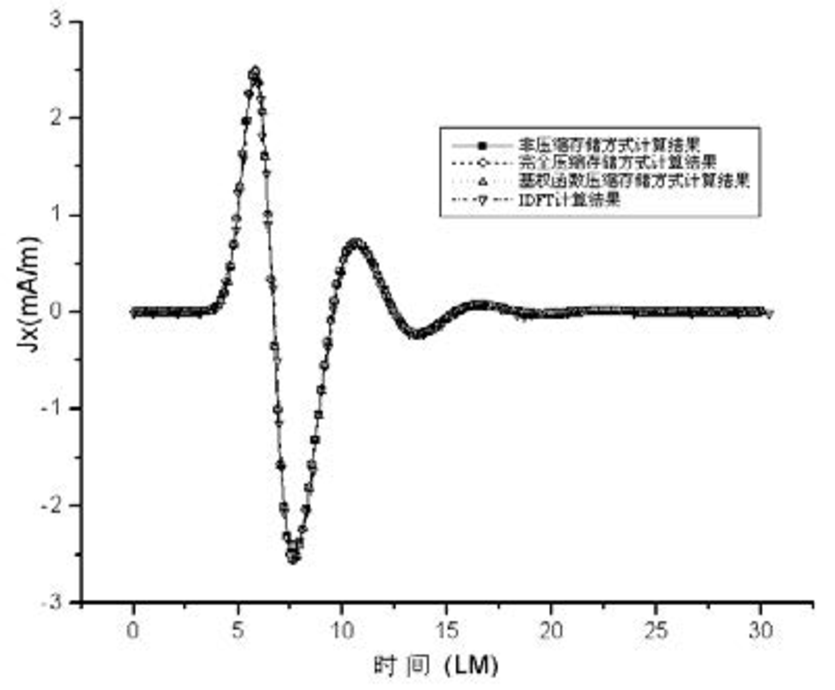
\includegraphics[width=6.77cm]{picd.pdf}
}
\subfloat[]{
    \label{pice}
    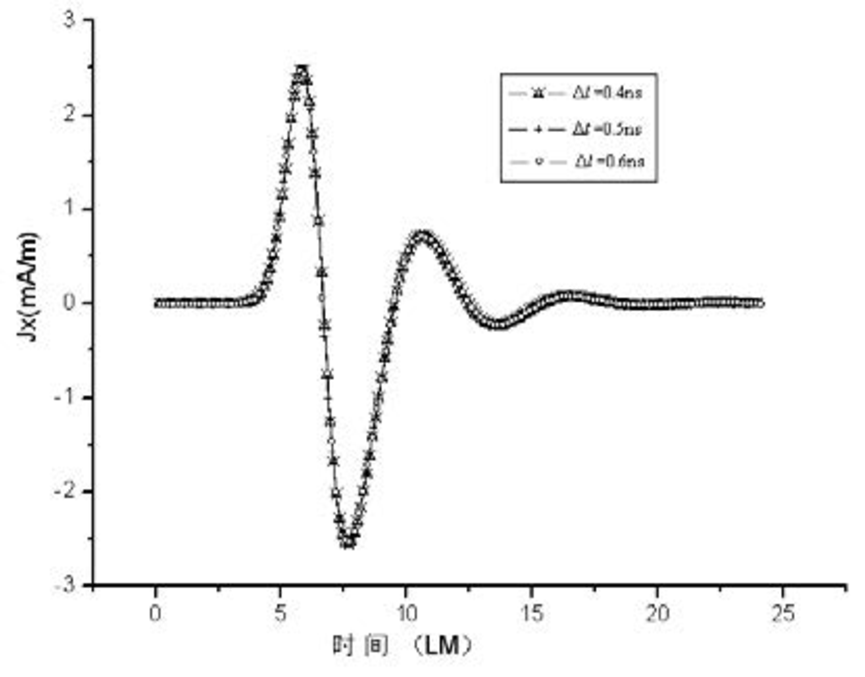
\includegraphics[width=7.04cm]{pice.pdf}
}
\caption{$2m\times 2m$的理想导体平板中心处感应电流$x$分量随时间的变化关系。(a)不同存储方式的计算结果与IDFT方法的结果比较;(b)不同时间步长的计算结果比较比较比较}
\label{fig2}
\end{figure}

由于时域混合场积分方程是时域电场积分方程与时域磁场积分方程的线性组合,因此时域混合场积分方程时间步进算法的阻抗矩阵特征与时域电场积分方程时间步进算法的阻抗矩阵特征相同。

\section{时域积分方程时间步进算法矩阵方程的求解}
\begin{theorem}
如果时域混合场积分方程是时域电场积分方程与时域磁场积分方程的线性组合。
\end{theorem}
\begin{proof}
由于时域混合场积分方程是时域电场积分方程与时域磁场积分方程的线性组合,因此时域混合场积分方程时间步进算法的阻抗矩阵特征与时域电场积分方程时间步进算法的阻抗矩阵特征相同。
\end{proof}
\begin{corollary}
时域积分方程方法的研究近几年发展迅速,在本文研究工作的基础上,仍有以下方向值得进一步研究。
\end{corollary}
\begin{lemma}
因此时域混合场积分方程时间步进算法的阻抗矩阵特征与时域电场积分方程时间步进算法的阻抗矩阵特征相同。
\end{lemma}

\section{本章小结}
本章首先研究了时域积分方程时间步进算法的阻抗元素精确计算技术,分别采用DUFFY变换法与卷积积分精度计算法计算时域阻抗元素,通过算例验证了计算方法的高精度。

\chapter{全文总结与展望}

\section{全文总结}
本文以时域积分方程方法为研究背景,主要对求解时域积分方程的时间步进算法以及两层平面波快速算法进行了研究。

\section{后续工作展望}
时域积分方程方法的研究近几年发展迅速,在本文研究工作的基础上,仍有以下方向值得进一步研究:

%\chapter{template}
This is the template of the chapter in split file.

\section{s1}
This is a section.

\subsection{sub1}
This is a subsection.

% misc

\thesisacknowledgement
在攻读博士学位期间,首先衷心感谢我的导师XXX教授


\thesisappendix

\chapter{中心极限定理的证明}

\section{高斯分布和伯努利实验}

% Uncomment to list all the entries of the database.
% \nocite{*}

\thesisbibliography{reference}

%
% Uncomment the following code to load bibliography database with native
% \bibliography command.
%
% \nocite{*}
% \bibliographystyle{thesis-uestc}
% \bibliography{reference}
%

\thesisaccomplish{publications}

\thesistranslationoriginal
\section{The OFDM Model of Multiple Carrier Waves}



\thesistranslationchinese
\section{基于多载波索引键控的正交频分多路复用系统模型}



\end{document}
